\documentclass[11pt]{article}
\usepackage{fullpage}
\usepackage[margin=2.5cm, bottom=3cm]{geometry}
\usepackage{amsmath,amsthm,amsfonts,amssymb,amscd}
\usepackage{mathrsfs}
\usepackage{fancyhdr}
\usepackage{multicol}
\usepackage{hyperref}
\usepackage{graphicx}
\usepackage[backend=biber]{biblatex}
\graphicspath{ {./../imgs/} }
\usepackage{bbm}

\addbibresource{baby_cry.bib}

\hypersetup{
colorlinks=true,
linkcolor=blue,
linkbordercolor={0 0 1},
citecolor=black
}

\linespread{1.25}
\pagestyle{fancyplain}
\headsep 1.5em
\headheight 14pt

\title{Image Segmentation Using Markov Random Fields: An Implementation}

\author{Jake Callahan, James Griffin, McKay Harward, Taylor Paskett, Isaac Robbins, Mingyan Zhao}

\begin{document}

\begin{abstract}
The goal of this project was to evaluate current use of Markov random fields in image segmentation, then to implement one of the more advanced methods. In this paper we discuss how we implemented the equations from a paper based on an unsupervised method that used metropolis Hastings algorithm to find the best parameters for the Markov random field as well as the best number of classes. In short, we coded up a hands-off method of segmenting an input image.
\end{abstract}

\section{Background and Motivation}
Image segmentation is one the the most important problems in machine learning today. Industries like medicine, transportation, and manufacturing have all been benefited by the rapid advances we have made in creating image segmentation systems. 
One of the most interesting and valuable fields of study is the area focused on unsupervised image segmentation methods. 
A powerful and accurate unsupervised image segmentation system would have applications in neural photo editing using introspective adversarial networks as well as in image recognition and other computer graphics applications. In this paper, we examine and implement Barker and Rayner's idea for using Markov random fields (MRFs) for unsupervised image segmentation [CITATION HERE].

 The idea for using Markov random fields for image segmentation has been around for a long time and much research has been done in this area, mostly focusing on supervised learning methods. 
 Most of this research centers around segmenting images based on pretraining a Markov random field on a class, and then estimating which pixels in a given image are most likely to be of that class. While this is useful, the more hands-off the approach the easier it is to apply to new scenarios as it does not require labeled data. 
 
 Unfortunately, research regarding hands-off applications is virtually nonexistent, and when we were able to find studies of unsupervised image segmentation methods, the mathematics required were far beyond the scope of this class.
 Other than Barker and Rayner's research, which was published in 2000, we could find no other papers studying the use of Markov random fields for unsupervised segmentation. 
 The main drawback of this unsupervised method is that it trades an initial investment of creating pertained Markov random fields for a computationally expensive algorithm using metropolis Hastings.
 However, because of the benefits this method provides--including learning not only the image classes but also how many classes to use--and because of the advances in computing power over the last 20 years, we believe that it is now valuable to revisit these methods in order to determine if applications are possible in the current world of machine learning.


\section{Data}
As an unsupervised method, the algorithm we outline below trains itself on each image it operates on. As such, we didn't need (or want) a large dataset to use in this project.
Instead, we curated a small corpus of images by hand that we believed would be useful in providing us information about how well our algorithm was training and making predictions. 
The image we used was a simple noisy grid of 16 different colored squares used by Barker and Rayner.
This served as a baseline to compare our results to those achieved in the paper.
We used a second simple image with only a few clear segments, which was used largely for testing the model as it was small and allowed us to run the model quickly.
Finally we used a few photographs to see the final results of our model.

\begin{figure}[!htb]
\begin{center}
\begin{multicols}{3}
    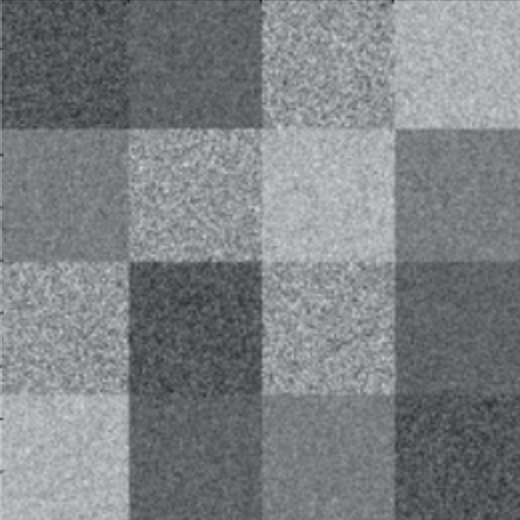
\includegraphics[height = \linewidth]{squares}\par
	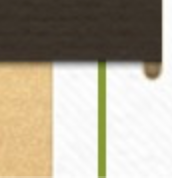
\includegraphics[height = \linewidth]{test}\
	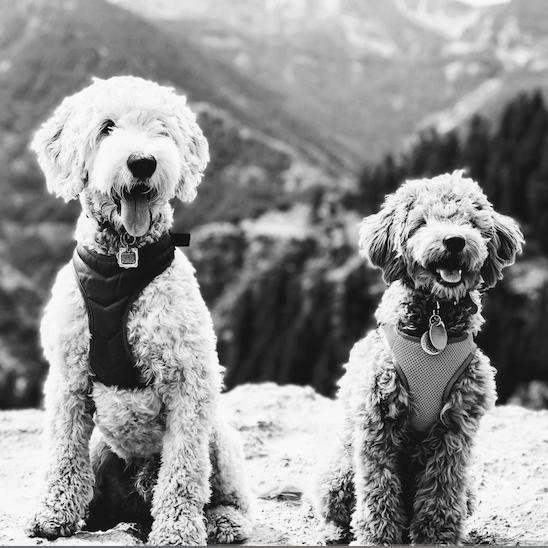
\includegraphics[height = \linewidth]{targetpractice}\par
\end{multicols}
\caption{The images used for training}
\end{center}
\end{figure}

\section{Methods}
Below is a simple overview of the algorithm proposed and then the modified algorithm we implemented.
A more in depth explanations of each step along with descriptions of the associated implementation and difficulties follow the algorithm.

\begin{enumerate}
	\item Randomly initialize the parameters for the MRF and number of classes
	\item Get the most likely segmentation given the MRF parameters
	\item Sample updated noise parameters $\mu$ and $\sigma$ for each class using Metropolis Hastings
	\item Sample updated MRF parameters $\beta_0$ and $\beta_1$ for each class using Metropolis Hastings
	\item Sample number of classes
	\item Repeat steps (2) - (5)
\end{enumerate}
The sampling method follows the same basic pattern: sample new parameters from their prior distributions, calculate an acceptance probability (or likelihood) for those parameters, and then use the Metropolis-Hastings algorithm to choose to accept/reject those parameters.

On the surface, this algorithm is simple. However, many of the equation definitions and notational choices were unclear and required extensive interpretation. 
Further, some of the equations as defined in the text suffered from under and overflow errors and thus required considerable reworking to be suitable for implementation. 
Sampling the number of classes was the most complex section of the paper and the notation was especially difficult to understand.
As such, we were unable to implement this step, but because the number of classes was a fixable parameter, this was not a significant issue.
Leaving this step out, we implemented the following method.
\begin{enumerate}
	\item Set the number of desired classes and randomly initialize the parameters for the MRF
	\item Get the most likely segmentation given the MRF parameters
	\item Sample updated noise parameters $\mu$ and $\sigma$ for each class using Metropolis Hastings
	\item Sample updated MRF parameters $\beta_0$ and $\beta_1$ for each class using Metropolis Hastings
	\item Repeat steps (2) - (4)
\end{enumerate}

\subsection{Variable Definitions}
We define the following variables to use in the various equations to follow:

\begin{itemize}
	\item $\Omega$: The image being classified
	\item $s$: A pixel of the image $\Omega$
	\item $Y$: The grayscale image intensities
	\item $y_{s}$: The grayscale intensity at pixel $s$ in the interval $(0,1]$
	\item $X$: The segmentation labels for the MRF
	\item $x_{s}$: The label to which pixel $s$ is assigned
	\item $\Lambda$: The set of class labels
	\item $\eta_{s}$: The set of 4 direct neighbors of pixel $s$
	\item $\Psi$: The parameter vector consisting of both noise and MRF parameters
	\item $\Theta_{c}$: The noise model parameter vector consisting of $\mu_{c}$ and $\sigma_{c}$
	\item $\beta_{c}^{(0)}$: The external field parameter
	\item $\beta_{c}^{(1)}$: The inter-pixel interaction strength parameter
	\item $T_{t}$: The annealing temperature at iteration $t$
	\item $n_{c}$: The number of pixels of class $c$
	\item $n_{(c, \eta)}$: Abusive notation explained in Section 3.3
\end{itemize}



\subsection{Segment the Image with the MRF}
With an initial set of random parameters to define our MRF, we needed to first find the probability of each pixel being in each class:
\begin{equation}
\begin{aligned}
p\left(x_{s} = c | y_{s}, \eta_{s}, \Psi_{c}\right) & \propto \\
&\frac{1}{\sqrt{2 \pi \sigma_{c}^{2} T_{t}}} \exp \left\{ -\frac{1}{T_{t}} \left[\frac{1}{2} \left(\frac{y_{s}-\mu_{c}}{\sigma_{c}}\right)^{2} + \left( \beta_{c}^{(0)} + \beta^{(1)} V(c, \eta_{s}) \right) \right] \right\}
\end{aligned}
\end{equation}
where $V(c, \eta)=\frac{1}{4} \sum_{t \in \eta}(c \oplus\left.x_{t}\right),$ where $\oplus$ is an operator defined to take the value -1 if its arguments are equal and 1 otherwise.

We then calculated the probabilities over the entire image for each class and took the argmax, thereby assigning each pixel to the class to which it most likely belongs.
The implementation of this process was relatively straightforward and required no adjustments to the equations.


\subsection{Update Noise Parameters}
The noise parameters $\mu_{c}$ and $\sigma_{c}$ are sampled using Metropolis-Hastings with the following likelihood:
\begin{equation}
\begin{aligned}
p\left(\mu_{c}, \sigma_{c} | Y, X\right) & \propto \prod_{s: x_{s}=c} p\left(y_{s} | \mu_{c}, \sigma_{c}\right) p_{r}\left(\mu_{c}\right) p_{r}\left(\sigma_{c}\right) \\
&=\frac{1}{\sigma_{c}\left(2 \pi \sigma_{c}^{2} T_{t}\right)^{n_{c}}} \exp \left\{-\frac{1}{2 T_{t}} \sum_{s: a_{s=c}}\left(\frac{y_{s}-\mu_{c}}{\sigma_{c}}\right)^{2}\right\}
\end{aligned}
\end{equation}

With a firm grasp on Metropolis-Hastings, we expected updating the noise parameters to be straightforward. However, the suggested $T_{t}$ from the paper was so large, we ran into immediate underflow errors during computation.
We soon realized the issue was the $n_{c}$ exponent in the denominator causing our underflow.
While segmenting a small 100 x 100 image into 4 classes, $n_{c}$ should be about 25,000 and possibly much larger.
This necessitated that we calculate the equation in a completely different form which we give below.

\begin{equation}
\begin{aligned}
p\left(\mu_{c}, \sigma_{c} | Y, X\right) & \propto \frac{1}{\sigma_{c}}\prod_{s: x_{s}=c} \frac{1}{2 \pi \sigma_{c}^{2} T_{t}} \exp \left\{-\frac{1}{2 T_{t}} \left(\frac{y_{s}-\mu_{c}}{\sigma_{c}}\right)^{2} \right\}
\end{aligned}
\end{equation}

This allowed us to avoid the exponent and the large sum, both of which could cause massive underflow by calculating a each part of the product individually.
Because this probability would be used only for the acceptance ratio $a$ in the Metropolis-Hastings algorithm, we extended this calculation one step further.

\begin{equation}
\begin{aligned}
a & = \frac{p\left(\mu_{c}^{new}, \sigma_{c}^{new} | Y, X\right)}{p\left(\mu_{c}, \sigma_{c} | Y, X\right)}\\ & \propto \prod_{s: x_{s}=c}  \frac{\frac{1}{2 \pi \sigma_{c}^{new2} T_{t}} \exp \left\{-\frac{1}{2 T_{t}} \left(\frac{y_{s}-\mu_{c}^{new}}{\sigma_{c}^{new}}\right)^{2} \right\}}{\frac{1}{2 \pi \sigma_{c}^{2} T_{t}} \exp \left\{-\frac{1}{2 T_{t}} \left(\frac{y_{s}-\mu_{c}}{\sigma_{c}}\right)^{2} \right\}}
\end{aligned}
\end{equation}

This allowed us to calculate the acceptance ratio for a single pixel before taking the product over all of the pixels of the specified class.
By doing so, we completely avoided underflow. However, we were only getting acceptance ratios of $0$ and $\infty$.
At first this concerned us but we realized that given model parameters, the individual ratios would be very similar (at least across each class) and thus for $a_{s} > 1$ taking the product would approach $\infty$ and for $a_{s} < 1$, the product would approach 0.
Having resolved this issue, we were able to update our noise parameters $\mu_{c}$ and $\sigma_{c}$ properly.

\subsection{Update MRF Parameters}
As in the previous step, the MRF parameters $\beta_{c}^{(0)}$ are sampled using Metropolis-Hastings with the following probability:

\begin{equation}
\begin{array}{l}
p\left(\beta_{c}^{(0)}, c \in \Lambda | X\right) \\
\quad=p\left(X | \beta_{c}^{(0)}, c \in \Lambda\right) p_{r}\left(\beta_{c}^{(0)}, c \in \Lambda\right) \\
\quad=\prod_{\left(c \in \Lambda, \psi_{\eta}\right)}\left(\frac{\exp \left(-\frac{1}{T_{t}}\left[\beta_{c}^{(0)}+\beta^{(1)} V(c, \eta)\right]\right)}{\sum_{i \in \Lambda} \exp \left(-\frac{1}{T_{t}}\left[\beta_{i}^{(0)}+\beta^{(1)} V(i, \eta)\right]\right)}\right)^{n_{(c, \eta)}} \\
\quad=\prod_{(c \in \Lambda)}\left(\frac{\exp \left(-\frac{1}{T_{t}}\left[\beta_{c}^{(0)}\right]\right)}{\sum_{i \in \Lambda} \exp \left(-\frac{1}{T_{t}}\left[\beta_{i}^{(0)}\right]\right)}\right)^{n_{c}} \\
\quad \times \prod_{(c \in \Lambda, \psi \eta)}\left(\frac{\exp \left(-\frac{1}{T_{t}}\left[\beta^{(1)} V(c, \eta)\right]\right) \sum_{i \in \Lambda} \exp \left(-\frac{1}{T_{t}}\left[\beta_{i}^{(0)}\right]\right)}{\sum_{i \in \Lambda} \exp \left(-\frac{1}{T_{t}}\left[\beta_{i}^{(0)}+\beta^{(1)} V(i, \eta)\right]\right.}\right)^{n_{(c, \eta)}}
\end{array}
\end{equation}

We immediately ran into the issue of the definition of the exponent $n_{(c, \eta)}$ that is used.
The paper defines this as $n_{(c, \eta)}=\#\left(s: x_{s}=c, \eta_{s}=\eta\right)$;
this notation is abusive and does not follow the paper's previously established notational conventions.
As written, this $n$ function takes in a class $c$ and a set of pixels $\eta$, then returns the number of pixels that have label $c$ and neighbors $\eta$. 
However, due to the way $\eta$ is defined at the beginning of the paper, each pixel will have a unique set of neighbors. 
 
Thus, this $n$ function will return a 1 if there is a pixel in class $c$ with the given set of neighbors $\eta$ and a $0$ if there is not a pixel in class $c$ with that exact set of neighbors. 
Then for each class, iterating over all $\eta_s$ with the $n$ function is equivalent to iterating over all $s: x_s = c$ with the indicator function $\mathbbm{1}(s,c)_{x_s = c}$.
This leads to probabilities corresponding to pixels such that $x_{s} \neq c$ being set to $1$ and essentially excluded from the product, so we remedied this equation as follows:

\begin{equation}
\begin{aligned}
p\left(\beta_{c}^{(0)}, c \in \Lambda | X\right) & = \prod_{s:x_{s} = c}\frac{\exp \left(-\frac{1}{T_{t}}\left[\beta_{c}^{(0)}+\beta^{(1)} V(c, \eta_{s})\right]\right)}{\sum_{i \in \Lambda} \exp \left(-\frac{1}{T_{t}}\left[\beta_{i}^{(0)}+\beta^{(1)} V(i, \eta_{s})\right]\right)}
\end{aligned}
\end{equation}

This greatly simplified the calculations for updating the MRF parameters  $\beta_{c}^{(0)}$.
We used the same method as described in Section 3.2 of calculating each of the individual acceptance ratios $a_{s}$ before taking the product over all the ratios.
A similar equation is proposed for the likelihood $p(\beta_{c}^{(1)}, c \in \Lambda | X)$. However, the paper states that the posterior density calculation for $\beta_{c}^{(1)}$ will not be proper under particular underlying label map configurations.
The paper fixes a value \textit{a priori} of $1.5$ for $\beta_{c}^{(1)}$.
We follow this practice in our approach.

\subsection{Number of classes}
The most difficult part of this paper involved sampling the number of classes.
The notation throughout this sections was very difficult to understand.
Below is the equation for the acceptance ratio for splitting a class $c$ into $c_{1}$ and $c_{2}$.

\begin{equation}
\begin{aligned}
\frac{p\left(X=x^{+}, \psi^{+}, k^{+} | Y=y\right)}{p(X=x, \psi, k | Y=y)} & \frac{1}{p_{\beta}\left(u_{1}\right) p_{\beta}\left(u_{2}\right) p_{\beta}\left(u_{3}\right)} \\
\times \frac{\partial\left(\Psi_{c 1}, \Psi_{c 2}\right)}{p(\text {segmentation})} &\left|\frac{1}{\partial\left(\Psi_{c}, u_{1}, u_{2}, u_{3}\right)}\right|
\end{aligned}
\end{equation}

Unfortunately, we were never able to work out the notation in a way that made enough sense to even try to implement this sampling.
However, this step only helps find the optimal number of classes for the segmentation, and omitting this step should not affect any other sampling or the performance of the algorithm as a whole.
With this step omitted from the algorithm, we simply specify the desired number of classes before running it.

\section{Results}


\section{Analysis}
Our methods turned out to be fairly effective. They don’t par with current state of the art technologies but they definitely do well for something done by a few undergraduate students in a single project, not research. The model we’ve created does a fairly decent job of segmenting images on par with what the original authors achieved, though sometimes in a few extra iterations. Looking at how it works, I do think it would work in a GAN for neural photo editing to maybe train the GAN to focus itself more closely on one area while keeping the rest of the image the same, but even with faster computers, it seems it still takes too long for any practical applications. Given enough computing power it can be used.

\section{Conclusion}
The initial intent of getting a completely unsupervised method of image segmentation using Markov Random Fields was successful and could probably be improved upon for efficiency. If given the opportunity to try image segmentation again, I would probably opt to use a neural network as they tend to require an initial investment of training time but can then be used to segment an image very quickly. Something we could do is have more informed priors for each parameters. We could also implement for color images (may be?)


\end{document}
